\section{Background and Motivation}\label{sec:background}

\subsection{LLM Serving and TTFT}

\begin{figure}[t!]
    \centering

    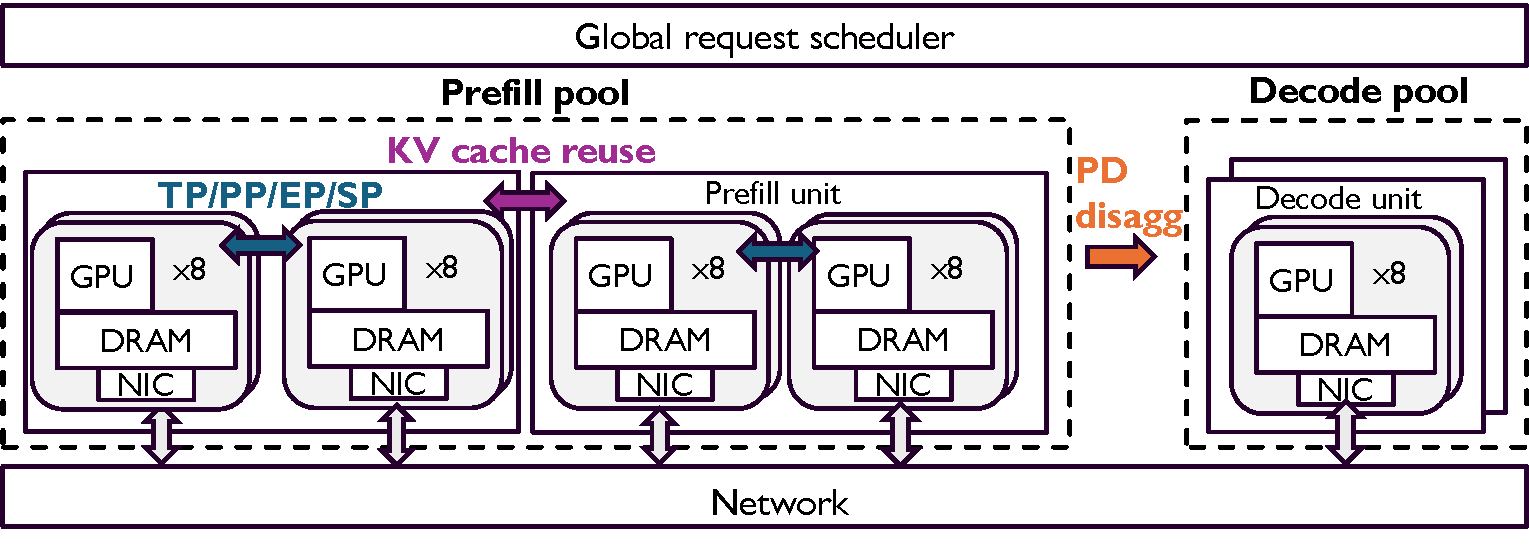
\includegraphics[width=\linewidth]{figures/moti/ServingOverview.pdf}
    \vspace{-0.5em}
    \caption{Illustration of LLM serving at scale.}
    \label{fig:bg:servingoverview}

\end{figure}


Large language models have become the foundation of modern AI services. These models are inherently autoregressive: the system first processes the entire prompt to generate the first token (the prefill stage), and then produces subsequent tokens iteratively using the accumulated KV cache (the decode stage). Performance is typically characterized by Time-to-First-Token (TTFT) for the prefill phase and Time-Between-Tokens (TBT) for the decode phase.

TTFT is a critical service-level objective (SLO) for many LLM applications. In interactive scenarios like chatbots and voice assistants, users expect an immediate initial response, and some studies indicate noticeable disengagement when latency exceeds a few hundred milliseconds and abandonment beyond seconds~\cite{vijaya2025aqua,liu2025m,kim2025seconds}. TTFT is also vital for automatic agentic frameworks, which rely on strict timeouts~\cite{langfuse,LiteLLM} for fault tolerance. A delayed first token triggers costly remedial actions such as service retries~\cite{Medium1,Medium2} or provider switching~\cite{notdiamond}. A recent report from Microsoft~\cite{ranganathan2025enhancing} reveals that the delayed first token is one of the primary source ($\sim 40\%$) of service failure (reported as timeout error), leading to revenue loss, higher support costs, and reputational risk.

As depicted in Fig.~\ref{fig:bg:servingoverview}, modern production systems~\cite{mooncake,deepseektech} scale out to clusters comprising thousands of nodes interconnected with high-bandwidth links, where each node contains multiple xPUs (\eg GPUs, TPUs, NPUs). Nodes are organized into individual serving units, each dedicated to host one model replica. Models are deployed using a combination of tensor~\cite{narayanan2021efficient}, pipeline~\cite{narayanan2019pipedream, alphaserve}, sequence~\cite{ringattention,wu2024loongserve,CP}, and expert parallelism~\cite{expertparallel,deepspeedMoE,deepseektech,comet}. To further optimize efficiency, recent work~\cite{distserve,splitwise,strati2024d,hu2024inference}  proposes \emph{prefill–decode disaggregation}, which assigns prefill tasks to compute-optimized devices and decode tasks to memory-rich devices, thereby accommodating their heterogeneous resource demands. In addition, \emph{KV cache reuse}~\cite{mooncakefast,hu2024memserve,cachedattention,cacheblend} has been introduced to amortize prefill costs across requests by transferring cached contexts between nodes.

\begin{figure}[t!]
    \centering
    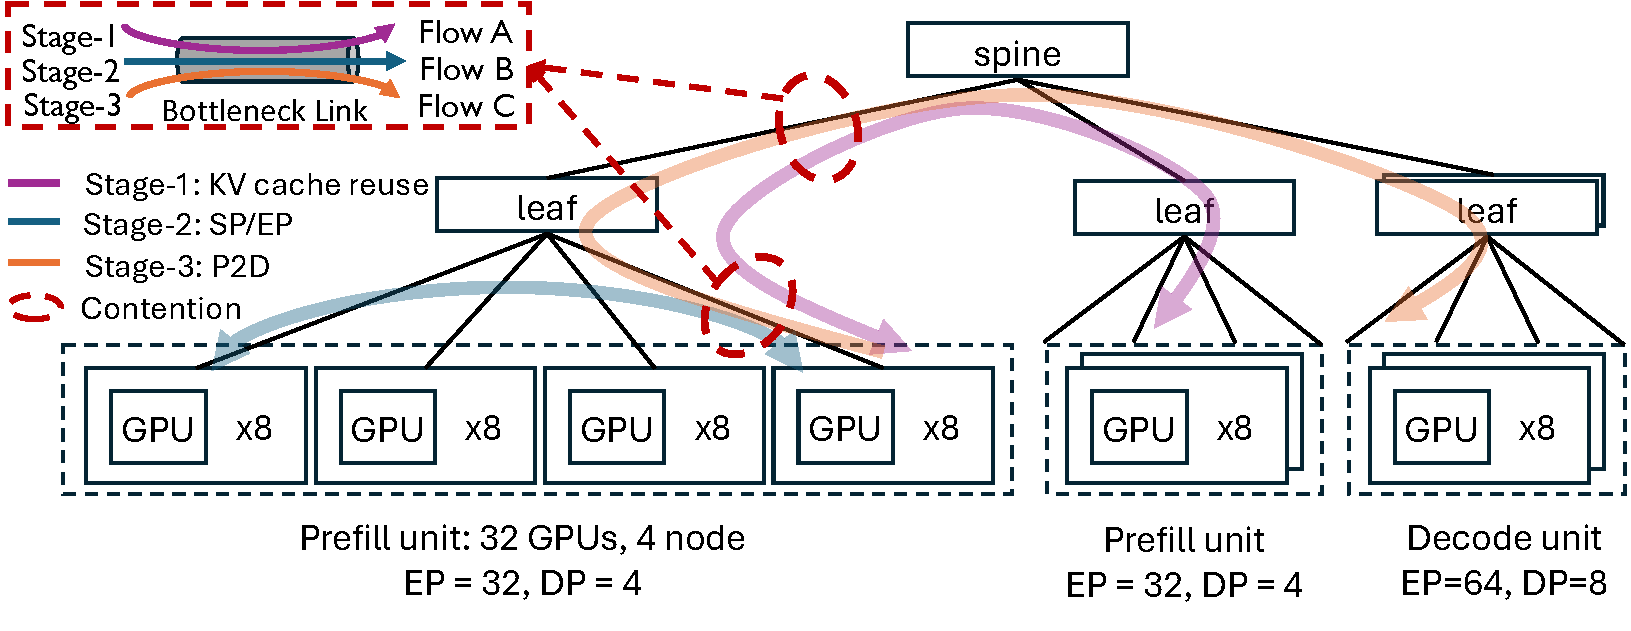
\includegraphics[width=\linewidth]{figures/moti/contentionmodel.pdf}
    \vspace{-0.5em}
\caption{An example illustrating communication contention in LLM serving systems: KV cache transfers (Stage~1 \& 3) and parallelism communication (Stage~2) compete for the same link bandwidth.}
    \label{fig:bg:contentionmodel}
\end{figure}

\begin{figure*}[ht!]
    \centering

    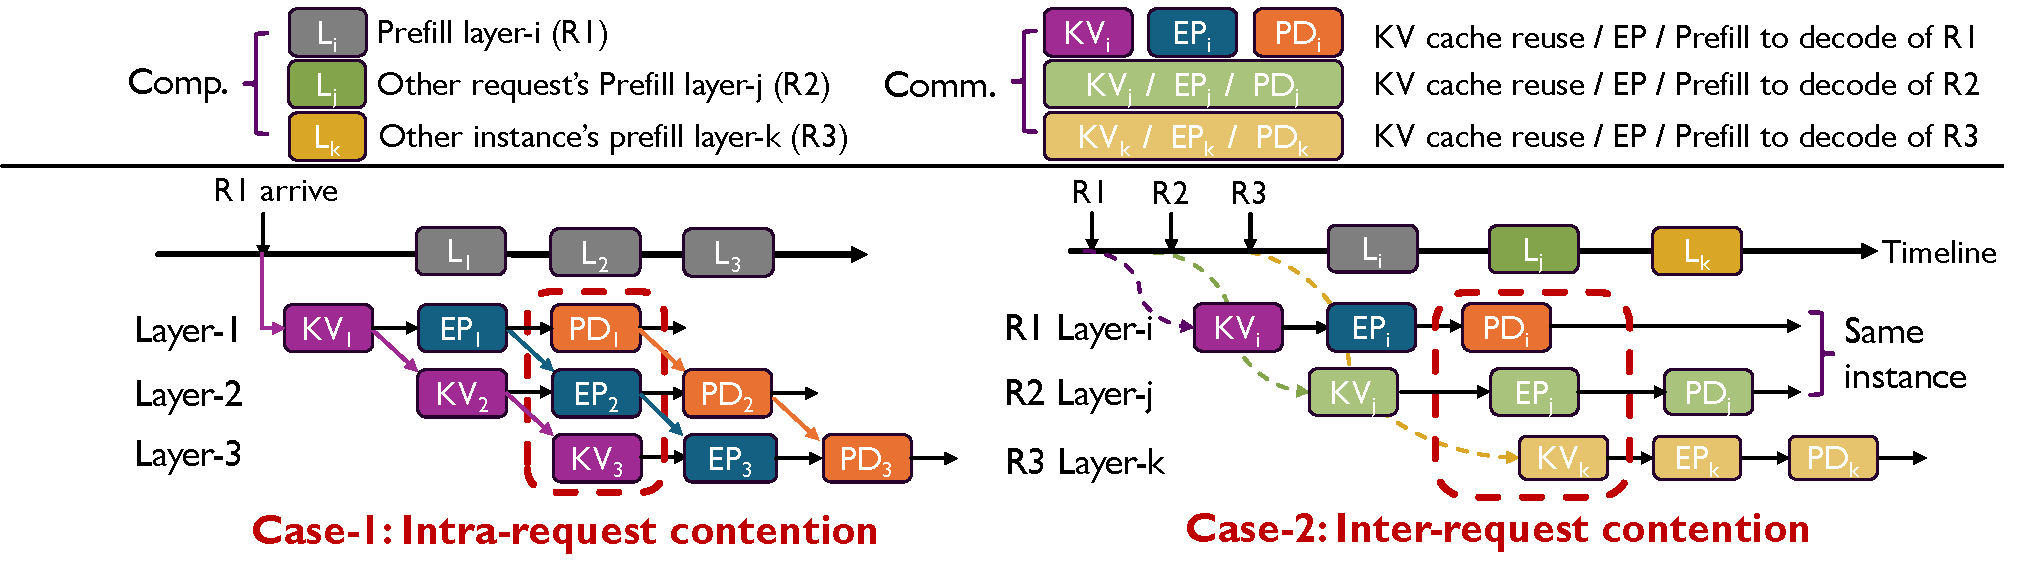
\includegraphics[width=0.9\linewidth]{figures/moti/contentioncase.pdf}

    \caption{Illustration of two primary forms of contention in LLM serving systems.}
    \label{fig:bg:contention}
\end{figure*}


\subsection{Contention Across Multi-Stage Communication}

Generating the first token in existing production systems (Fig. \ref{fig:bg:servingoverview}) consists of multi-stage communications:
\begin{enumerate}[label=\(\bullet\),leftmargin=*]
    \item \textbf{Stage~1: KV-cache reuse}: fetches reusable KV-cache blocks from remote prefill unit;
    \item \textbf{Stage~2: Collective communication}: exchanges intermediate activations across devices via model parallelism;
    \item \textbf{Stage~3: Prefill-to-Decode (P2D) transfer}: delivers the full KV-cache history to the decode unit \footnote{Mainstream open-source serving frameworks~\cite{vllm_pd_2025,sglang_pd_2025,dynamo_pd_2025} explicitly incorporate Stage~3 latency into the TTFT metric.}.
\end{enumerate}

Prior literature has highlighted the substantial overhead of individual stages, noting that collective communication (e.g, all-to-all, etc.) occupy 40--60\% of end-to-end latency \cite{linaatc,comet,li2025optimizing,CP} and KV-cache movement contributes a non-trivial share~\cite{cachegen,mooncake,chen2024kvdirect,li2025flowkv,yoon2025tract}. In this paper, we further identify a critical yet underexplored problem: collective communication and KV-cache movement frequently overlap in time and contend for shared network bandwidth. Fig.~\ref{fig:bg:contentionmodel} illustrates the spatial location of contention: KV-cache transfers (Stage~1\&3) and collective communication (Stage~2) traverse shared physical interconnects. This spatial co-location creates two primary forms of contention, as shown in Fig.~\ref{fig:bg:contention}:
\begin{itemize}[leftmargin=*]
    \item \textbf{Intra-request contention} occurs when communication flows interfere within a single request. Specifically, layer-wise KV-cache transfers (Stage~1\&3) compete directly with the ongoing collective communication on other layers (Stage~2) for shared link bandwidth.
    \item \textbf{Inter-request contention} arises when concurrent requests from different prefill units interfere, resulting in frequent link competition in the switch links. Moreover, driven by skewed block popularity, multiple prefill units may converge on a single remote \textit{victim unit} to fetch ``hot'' KV blocks, causing contention between the victim unit's local collective communication (Stage~2) and remote KV-cache fetching on its NIC bandwidth (Stages~1\&3).
\end{itemize}

\begin{figure}[t]
    \centering
    \begin{subfigure}[t]{0.48\linewidth}
        \centering
        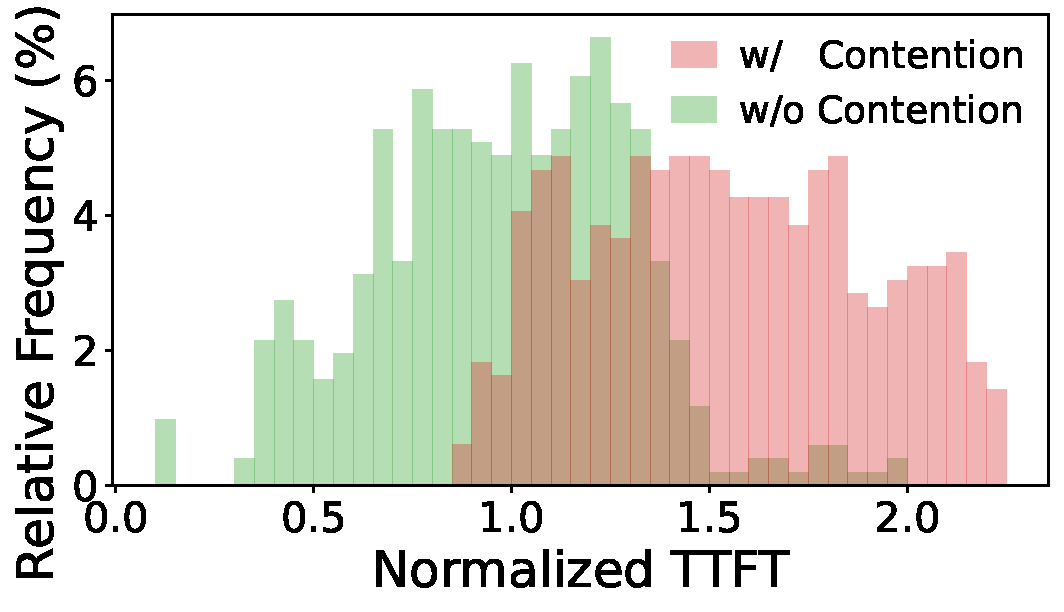
\includegraphics[width=\linewidth]{figures/moti/ttft_norm_hist_percent.pdf}
        \caption{Impact of contention on end-to-end TTFT.}
        \label{fig:moti:ttft}
    \end{subfigure}
    \hfill
    \begin{subfigure}[t]{0.48\linewidth}
        \centering
        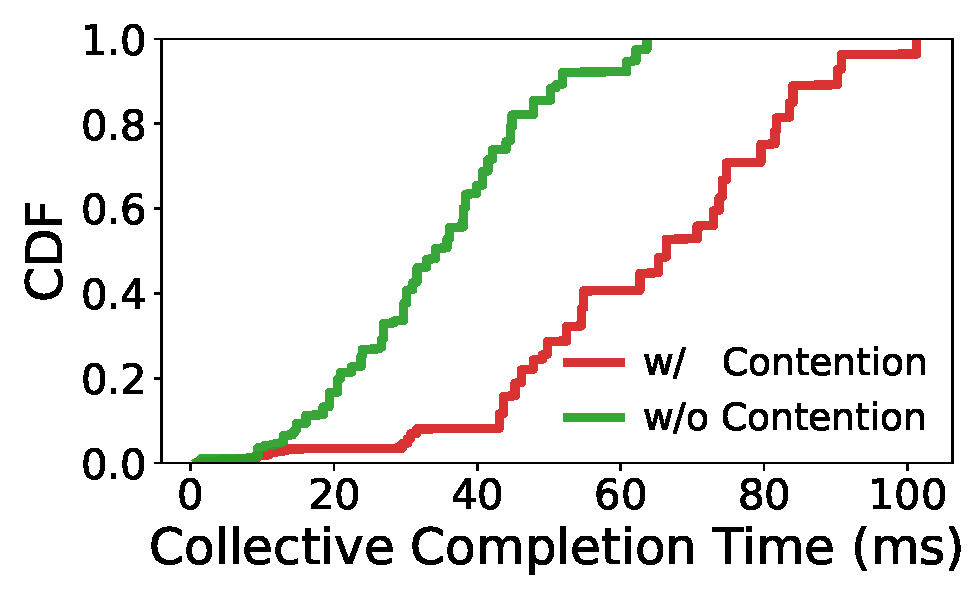
\includegraphics[width=\linewidth]{figures/moti/alltoall_8_cct_cdf.pdf}
        \caption{Impact of contention on all-to-all latency.}
        \label{fig:moti:cct}
    \end{subfigure}
    \hfill

    \caption{[Testbed] Impact of communication contention on Mixtral 8x7B model.}

    \label{fig:moti:contentionimpact}
\end{figure}


To quantify the performance degradation caused by such interference, we conduct measurements on a 16-GPU prefill cluster (50 Gbps/GPU) hosting two serving instances ($TP=1, EP=8$). We use QwenB-agent, an agent workload from production-derived Qwen traces~\cite{qwen_bailian_traces}, with average sequence length 1k tokens, 65\% prompt reuse, and per-GPU request rate 1 req/s; the full testbed setup is described in Sec.~\ref{sec:evaluation:testbed}. We evaluate the impact of contention on two metrics: end-to-end TTFT and collective communication time (CCT) of All-to-All operations (aggregating Dispatch and Combine phases). Specifically, we perform a comparative analysis between an ideal baseline (\textit{w/o contention}) and a realistic serving scenario (\textit{w/ contention}). Fig.~\ref{fig:moti:ttft} illustrates the TTFT distribution. The results reveal that, under contention, the overall TTFT is prolonged by nearly $50\%$. We attribute this inflation primarily to the latency degradation in All-to-All communication on the critical path, whose CCT nearly doubles ($1.8\times$) due to contention with concurrent KV-cache operations (as shown in Fig.\ref{fig:moti:cct}). This substantial slowdown confirms that network contention is a major source of performance variability in the prefill phase.

\subsection{Limitation of Existing Work}
The previous analysis identifies unmanaged multi-stage communication contention as a primary source of TTFT violations. We categorize existing approaches into two groups: recent system-level communication optimizations and conventional scheduling algorithms. As detailed below, they both fall short in coordinating such contention due to the lack of a holistic view of multi-stage dependencies.

\parab{Stage-agnostic flow scheduling.} Conventional datacenter scheduling disciplines manage flows or coflows individually to optimize network metrics, such as flow/coflow completion time or deadline satisfaction. However, these objectives are misaligned with end-to-end application goals (e.g., TTFT attainment), because TTFT is jointly determined by flows across multiple interdependent stages. Consequently, these approaches inevitably over-prioritize slack-rich flows while starving the critical transfers required to unlock downstream computation, ultimately degrading TTFT SLO attainment.

\parab{Specialized optimization for isolated stages.}
We notice some distinct efforts optimize isolated stages, specifically targeting collective communication via algorithm synthesis~\cite{shah2023taccl,liu2024rethinking,kim2024tccl,cao2025syccl}, parameter tuning~\cite{xu2025autoccl}, and overlapping~\cite{deepseektech,comet,zheng2025triton,zheng2025tilelink}, or KV-cache transfers via pipelined prefetching \cite{splitwise,mooncakefast} and block coalescing \cite{strati2024d,chen2024kvdirect,li2025flowkv}. However, these mechanisms often pursue conflicting objectives. Many achieve speedups by increasing communication concurrency to hide latency, yet none coordinates this concurrency across communication types. As a result, even with these optimizations, collective communication and KV-cache transfers often interfere with one another, which instead amplifies contention.
